\documentclass
[handout]
{beamer}


%%
%%
%%
% From http://tex.stackexchange.com/questions/2072/beamer-navigation-circles-without-subsections
% Solution #2 or 3:
% \usepackage{etoolbox}
% \makeatletter
% % replace the subsection number test with a test that always returns true
% \patchcmd{\slideentry}{\ifnum#2>0}{\ifnum2>0}{}{\@error{unable to patch}}%
% \makeatother
% Solution #1:
\usepackage{remreset}% tiny package containing just the \@removefromreset command
\makeatletter
\@removefromreset{subsection}{section}
\makeatother
\setcounter{subsection}{1}


\usepackage{etex}
\usepackage{pgf}
\usepackage{tikz}
\usepackage{url}
\usepackage{amsmath}
\usepackage{color}
% \definecolor{red}{rgb}{1,0,0}
\usepackage{ulem}
% \usepackage{booktabs}
\usepackage{colortbl,booktabs}
\renewcommand*{\thefootnote}{\fnsymbol{footnote}}
\usepackage{fancybox}
\usepackage[framemethod=TikZ]{mdframed}
\mdfdefinestyle{FactStyle}{%
  outerlinewidth=0.5,
  roundcorner=1pt,
  leftmargin=1cm,
  linecolor=blue,
  outerlinecolor=blue!70!black,
  backgroundcolor=yellow!40
}
\usepackage{cancel}

  \newcommand\Warning{%
    \makebox[2.4em][c]{%
      \makebox[0pt][c]{\raisebox{.2em}{\Large!}}%
      \makebox[0pt][c]{\color{red}\Huge$\bigtriangleup$}}}%

\usepackage{stackengine}
\usepackage{scalerel}
\usepackage{xcolor}
  \newcommand\dangersign[1][2ex]{%
    \renewcommand\stacktype{L}%
    \scaleto{\stackon[1.3pt]{\color{red}$\triangle$}{\tiny !}}{#1}%
  }



\usepackage{dcolumn}
\newcolumntype{d}[1]{D{.}{.}{#1}}

% From
% http://tex.stackexchange.com/questions/109900/how-can-i-box-multiple-aligned-equations
\usepackage{empheq}
\usepackage{tcolorbox}  \newtcbox{\othermathbox}[1][]{%
  nobeforeafter, tcbox raise base, 
  colback=black!10, colframe=red!30, 
  left=1em, top=0.5em, right=1em, bottom=0.5em}

\newcommand\blue{\color{blue}}
\newcommand\red{\color{red}}
\newcommand\green{\color{green!75!black}}
\newcommand\purple{\color{purple}}
\newcommand\bluegreen{\color{blue!75!green}}
\newcommand\orange{\color{orange}}
\newcommand\redgreen{\color{red!50!green}}
\newcommand\grey{\color{black}}
\newcommand\gap{\vspace{.1in}}
\newcommand\nb{${\red\bullet}\ $}
\newcommand\halfgap{\vspace{.05in}}
\newcommand\divideline{\line(1,0){352}}
\usepackage{marvosym} % for \Smiley

\newcommand{\bluealert}[1]{{\blue\textbf{#1}}}

% \usepackage{beamerthemesplit} %Key package for beamer
\usetheme{Singapore}
% \usetheme{Szeged}
% \usetheme{Garfield}
% \usetheme{CambridgeUS}
% \usenavigationsymbolstemplate{} %Gets rid of slide navigation symbols


\setbeamercolor{separation line}{use=structure,bg=structure.fg!50!bg}
% \begin{beamercolorbox}[colsep=0.5pt]
%   {upper separation line foot}
% \end{beamercolorbox}



\makeatletter
\setbeamertemplate{footline}
{
  \leavevmode%
  \hbox{%
% \begin{beamercolorbox}[colsep=0.5pt]
%   {upper separation line foot}
% \end{beamercolorbox}


  \begin{beamercolorbox}[wd=.5\paperwidth,ht=2.25ex,dp=2ex,colsep=0.5pt]%
    {upper separation line foot}
    \usebeamerfont{author in head/foot}%
    \hspace*{2ex}\insertshortdate:\ \insertshorttitle
  \end{beamercolorbox}%
  \begin{beamercolorbox}[wd=.5\paperwidth,ht=2.25ex,dp=2ex,right]{title in head/foot}%
    \usebeamerfont{title in head/foot}
    {\insertshortauthor}\hspace*{2ex}
  \end{beamercolorbox}}%
  % \begin{beamercolorbox}[wd=.333333\paperwidth,ht=2.25ex,dp=2ex,right]{date in head/foot}%
  %   \usebeamerfont{date in head/foot}\insertshortdate{}\hspace*{2em}
  %   \insertframenumber{} / \inserttotalframenumber\hspace*{2ex} 
  % \end{beamercolorbox}%
  \vskip0pt%
}
\makeatother

\usetikzlibrary{decorations.markings}
\usetikzlibrary{arrows}


\title{Final Exam Review}
\author{Peter Garfield, UCSB Mathematics}
\date{March 15, 2017}
%\institute{}


\useinnertheme{default}

\usefonttheme{serif}
% \usecolortheme{rose}
% \usecolortheme{whale}
% \usecolortheme{orchid}
\usecolortheme{crane}
% \usecolortheme{dolphin}


%TEMPLATE
\setbeamertemplate{navigation symbols}{}

\setbeamertemplate{note page}[compress]

\setbeamertemplate{frametitle}{
  \vspace{0.5em}
  % \begin{centering}
  {\huge\blue\textbf{\textmd{\insertframetitle}}}
  \par
  % \end{centering}
}

% From http://tex.stackexchange.com/questions/7032/good-way-to-make-textcircled-numbers:
\newcommand*\circled[1]{\tikz[baseline=(char.base)]{\node[shape=circle,draw,fill=orange,inner sep=1pt] (char) {#1};}} 
% \renewcommand{\labelenumi}{\circled{\textbf{\arabic{enumi}}}}

\let\olddescription\description
\let\oldenddescription\enddescription
\usepackage{enumitem}
\let\description\olddescription
\let\enddescription\oldenddescription

% \usepackage[loadonly]{enumitem}
\setlist[enumerate,1]{label=\colorbox{orange}{\arabic*.},font=\bfseries}
%\setlist[enumerate,2]{label=\colorbox{blue!25}{(\alph*)},font=\bfseries}
% \setlist[enumerate,1]{label=\arabic*.,font=\bfseries}
\setlist[itemize,1]{label=\red$\bullet$}
\setlist[itemize,2]{label=\blue$\bullet$}

\newcommand\answer[1]{\fbox{#1}}
% \renewcommand\answer[1]{}

\newcommand{\antilog}{\operatorname{antilog}}







\title{}
\title{Limits and Stuff}
\date{April 12, 2022}


\begin{document}
\small

\section*{Administration}

\frame{
  \frametitle{}
  {\Huge{}Welcome Back!}\\[.5em]

  {\Huge{}Differential Calculus}
  \vfill
  {\Large{}Instructor:}\\
  \ \hspace*{0.2in} Nathan Schley ({\it Sh}+{\it lye}), \url{schley@math.ucsb.edu}\\
  \ \hspace*{0.2in} South Hall 6701
  \\[0.5em]

  {\Large{}Office Hours:}\\
  \ \hspace*{0.2in} T R 11-11:50, T 3:45-4:35 Details on Gauchospace. 
  \bigskip

  \copyright\ 2022\ Daryl Cooper, Peter M.\ Garfield, Ebrahim Ebrahim \& Nathan Schley\\
  Please do not distribute outside of this course.
  \vfill

}

\frame{
  \frametitle{Midterm 1: Next Tuesday in class}

  {\Large\color{blue}Bring:}
  \begin{itemize}
  \item A pen or \alert{sharp} pencil.
  \item A $3"\times5"$ notecard (both sides!).
  \item Student ID (so we can make sure it's you)
  \end{itemize}
  \bigskip

  {\Large\color{red}Don't bring:}
  \begin{itemize}
  \item A calculator
  \end{itemize}
  \bigskip

  {\Large\color{orange}Please Be Early!}
  \smallskip

  See textbook for sample exam questions.


}


\frame{
  \frametitle{Warm-up}

  {\large {\blue $\log_3(9) = ?$} means {\blue ``How many times do we need to triple 1 to get 9?''} }
  \pause   
  \begin{itemize} 
  \item $\log_3(9) = $ \pause \ \ \fbox{2}
  \pause
  \item $\log_3(81) = $ \pause \ \ \fbox{4}
  \pause
  \item $\log_3(1) = $ \pause \ \ \fbox{0}
  \pause
  \item $\log_3(\frac{1}{3}) = $ \pause \  \fbox{-1}
  
  \end{itemize}
  
  
  

} 

\frame{
  \frametitle{Warm-up Part II}

  {\large \blue Let's try it with decupling! }
  \pause   
  \begin{itemize} 
  \item $\log_{10}(100) = $ \pause \ \ \fbox{2}
  \pause
  \item $\log_{10}(1000) = $ \pause \ \ \fbox{3}
  \pause
  \item $\log_{10}(1) = $ \pause \ \ \fbox{0}
  \pause
  \item $\log_{10}(.0001) = $ \pause \  \fbox{-4}
  \pause
  \item $\log_{10}($100000000000000000000000000000000000000\\00000000000000000000000000000000000000000000\\000000000000000000$) = $ \pause \ \ \fbox{100} \pause \\ 
  
  \end{itemize}
  
  
}  


\frame{
  \frametitle{Warm-up Part III}

  {\large \blue Closeness }
  \pause   
  \begin{itemize} 
  \item As $x$ gets close to 0, $2+x$ gets close to... \pause \ \ \fbox{2}
  \item As $x$ gets close to 0, $5+2x$ gets close to... \pause \ \ \fbox{5}
  \item As $x$ gets close to 0, $3+x^2$ gets close to... \pause \ \ \fbox{3}
  \item As $x$ gets close to 3, $5x$ gets close to... \pause \ \ \fbox{15}
  \item As $x$ gets close to 2 and $y$ gets close to 3, $\frac{x}{y}$ gets close to... \pause \ \ \fbox{$\frac{2}{3}$}
  
  \end{itemize}
  
  
}  


\section*{Error \& Limit}

\frame{
  \frametitle{\S5.1: Error and Limit}

  Suppose the ``real'' answer is $10$, but your approximate answer is $9.5$
  \begin{empheq}[box=\othermathbox]{equation*}
    \text{{\red error}} 
    = \text{(real answer)} - \text{(approximate answer)}
  \end{empheq}

  In example $\text{\red error} = 10-9.5 = 0.5$
  \pause

  \begin{empheq}[box=\othermathbox]{equation*}
      \text{{\blue \% error}}
      = \left(\frac{\text{error}}{\text{real answer}}\right)\ \times\ 100\% 
  \end{empheq}

  In other words it is the error expressed as a {\blue percentage} of the real answer.\\
  Often this is what matters.
  % {\green discuss} 
  \pause

  % Often we take {\bf absolute value} to make the error positive.
  \gap

  \begin{enumerate}
  \item You have \$50 in you pocket but YOU THINK you have only
    \$40. What is the {\blue percentage error}? 
    \begin{equation*}
      \text{A} = 10\%
      \qquad 
      \text{B}=20\%
      \qquad 
      \text{C} = 25\%
      \qquad 
      \text{D} = 40\%
      \qquad 
      \text{E} = 50\%
      \pause
      \qquad 
      \answer{B}
    \end{equation*}
  \end{enumerate}
  % Because ${\red error}\ =\ 20-10=10.$ So {\blue percentage error} is this as a percentage of $20$ in other words $(10/20) \times 100\% = 50\%.$


}

\frame{
  \frametitle{Limits}

  Imagine you calculate more and more accurate approximations to a
  {\color{blue}real answer} that you don't know. 

  \begin{minipage}{0.3\linewidth}
    \begin{align*}
      x_1 & = 1.3\\ \pause
      \uncover<2->{x_2 & = 1.33}\\ 
      \uncover<3->{x_3 & = 1.333}\\ 
      \uncover<4->{x_4 & = 1.3333}\\
      \uncover<5->{%
          & \ \ \vdots \\
          & = \text{\blue real answer???} 
            }
    \end{align*}
  \end{minipage}


  \uncover<6->{These numbers get ever closer to $1.3333\cdots\ =\ 4/3$.}

  \uncover<7->{This is the {\color{blue}real answer}. }
  \uncover<8->{%
    The {\color{blue}limit} of this sequence is $4/3$:
    \begin{equation*}
      {\blue \lim_{{\red n}\to{\orange \infty}}\ {\purple x}_{\red n}}\ 
      = 4/3
    \end{equation*}
    Read aloud as ``{\blue The limit as $\red n$ goes to {\orange
        infinity} of ${\purple x}_{\red n}$ is $4/3$}.'' 
  }

}

\frame{ 
  \frametitle{Guessing Limits}
  
  To work out ({\blue guess}) a limit (when $\red n$ goes to {\orange
    infinity}) imagine plugging into the formula a REALLY BIG value
  for $\red n$ like a thousand, or a million, or\ldots

  \begin{enumerate}
    \setcounter{enumi}{1}
  \item $\displaystyle\lim_{{\red n}\to{\orange \infty}}\ \left(\frac{1}{\red n}\right)\ =\ ?$
    \bigskip

    \begin{equation*}
      \text{A} = \frac{1}{\red n}
      \qquad 
      \text{B} = 0
      \qquad 
      \text{C} = 1
      \qquad 
      \text{D} = \frac{1}{\orange \infty}
      \qquad 
      \text{E} = {\orange \infty}
      \pause
      \qquad
      \answer{B}
    \end{equation*}
    \gap

    % Because when you plug in a really big number for $\red n$ and
    % work out $1/\red n$ the answer is tiny. The bigger you make
    % $\red n$ the tinnier the answer.\pause 


    \item $\displaystyle\lim_{{\red n}\to\orange \infty}\ \left(\frac{\red n}{{\red n}+3}\right)\ =\ ?$
      \bigskip
      
      \begin{equation*}
        \text{A} = 0
        \qquad 
        \text{B} = 1/3
        \qquad 
        \text{C} = 1
        \qquad 
        \text{D} = 1/4
        \qquad 
        \text{E} = {\orange \infty}/({\orange \infty} + 3).
        \pause
        \qquad
        \answer{C}
      \end{equation*}

      % Because when you plug in a really big number for $\red n$ and
      % work out ${\red n}/({\red n}+3)$ the answer is really close to
      % $1.$ The bigger you make ${\red n}$ the closer the answer is to
      % $1.$ \pause

      \gap

      % When ${\red n}$ is {\huge REALLY BIG}, adding $3$ to it does
      % not really make {\blue any significant difference}. So it is
      % like working out ${\red n}/{\red n}$ since the $+3$ is not
      % important.

  \end{enumerate}



}

\frame{
  \frametitle{More Guessing Limits}

  \begin{enumerate}
    \setcounter{enumi}{3}
  \item $\displaystyle\lim_{{\red n}\to\orange\infty}\ \left( \frac{2{\red n}+5}{9{\red n}+71}\right)\  =\ ?$
    \bigskip

    \begin{equation*}
      \text{A} = \frac{5}{71}
      \qquad 
      \text{B} = \frac{2}{71}
      \qquad 
      \text{C}=\frac{5}{9}
      \qquad 
      \text{D} = \frac{2}{9}
      \qquad 
      \text{E} = \frac{2{\orange \infty}}{9{\orange \infty}}
      \pause
      \qquad
      \answer{D}
    \end{equation*}

    % Because when you plug in a really big number for ${\red n}$ and work
    % out $(2{\red n}+5)/(9{\red n}+72)$ the answer is really close to
    % $2/9.$ \pause The bigger you make ${\red n}$ the closer the answer is
    % to $2/9.$ \pause

    % \vspace{.05 in} When ${\red n}$ is REALLY BIG, adding $5$ or $71$ to
    % it {\blue does not really make any significant difference}. So it is
    % like working out $(2{\red n})/(9{\red n})$ and this is just
    % $2/9.$\pause


  \end{enumerate}
  \vspace{.1in}
  \gap

  For homework, you can use a calculator and plug in really big values
  for ${\red n}$ then guess. For example if you plug in
  ${\red n}=1000000$ and get the answer $16.{\orange 0000361}$ you
  guess the limit is really $16.$\pause
  \gap 

  For engineering, calculus students learn lots of tricks to work out
  limits. In this class we don't do that. Just UNDERSTAND the main
  idea.  

}


\frame{
  \frametitle{Even More Guessing Limits}
  \begin{enumerate}
    \setcounter{enumi}{4}
  \item 
    $\displaystyle\lim_{{\red n}\to\orange \infty}\left(\frac{2{\red n}+17}{5{\red n}+8}\right)\ =\ ?$
    \bigskip

    \begin{equation*}
      \text{A} = \frac{2}{5}
      \qquad 
      \text{B} = \frac{17}{5}
      \qquad 
      \text{C} = \frac{2}{8}
      \qquad 
      \text{D} = \frac{17}{8}
      \qquad 
      \text{E} = \frac{19}{13}
      \pause
      \qquad 
      \answer{A}
    \end{equation*}
    % When {\red n} is big can ignore the +17 and +8.  This leaves $2{\red n}/5{\red n}=2/5$\pause
    \gap

  \item
    $\displaystyle\lim_{{\red n}\to\orange \infty}\left(3+\frac{1}{{\red n}}\right)\ =\ ?$
    \bigskip

    \begin{equation*}
      \text{A} = 1
      \qquad 
      \text{B} = 3
      \qquad 
      \text{C} = 0
      \qquad 
      \text{D} = \frac{1}{3}
      \qquad 
      \text{E} = {\orange\infty}
      \pause
      \qquad 
      \answer{B}
    \end{equation*}
    % When {\red n} is very big $1/{\red n}$ is almost $0.$
    \gap

  \end{enumerate}


}
\frame{
  \frametitle{More: Spot The Difference!}

  \begin{enumerate}
    \setcounter{enumi}{6}
  \item 
    $\displaystyle{\blue \lim_{{\orange x}\to {\red 1}}}\ \left(\frac{{\orange x}-1}{{\orange x}^2-1}\right)$\pause\
    ${=\ \dfrac{1}{2}}$
    \bigskip
    \pause

  \item
    $\displaystyle\lim_{x\to{\color{red}1}}\left(\frac{x+3}{x^2+1}\right)\ =\ ?$
    \bigskip

    \begin{equation*}
      \text{A} = 3
      \qquad 
      \text{B} = 1
      \qquad 
      \text{C} = 4
      \qquad 
      \text{D} = 2
      \qquad 
      \text{E} = 0
      \qquad
      \pause\answer{D}
    \end{equation*}
    \pause
    \gap

    % In this case we can actually plug in $x=\red 1$ without getting
    % $0/0$ and this gives $(1+3)/(1^2+1)=4/2=2.$ \pause If we plug in a
    % number very close to $\red 1$ like $1.0001$ we will get an answer
    % very close to $2.$ \pause The whole limit thing is only {\blue
    % tricky} {\red when you can't plug in the final value for $x$}
    % (This happens if $x\to\infty$ 'cos you can't plug in $\infty.$ It
    % also happens if you get $0/0$ when you try).

  \item
    $\displaystyle\lim_{x\to{\color{red}0}}\left(\frac{3x+x^2}{2x}\right)\ =\ ?$
    \bigskip


    \begin{equation*}
      \text{A} = 0
      \qquad 
      \text{B} = \frac{0}{0}
      \quad 
      \text{C} = \frac{1}{0}
      \qquad 
      \text{D} = \frac{1}{2}
      \qquad 
      \text{E} = \frac{3}{2}
      \qquad
      \pause\answer{E}
    \end{equation*}
    % When $x$ is very small like $x=0.01$ then $x^2=0.0001$ is much smaller.\\
    % So {\blue ignore $x^2$  in comparison to $3x$  when $x$ is very small}
    % $$\text{when x is small}\qquad\qquad\qquad\frac{3x+x^2}{2x}\approx \frac{3x}{2x}=\frac{3}{2}.$$

    % {\grey  take it to the limit clip  }
  \end{enumerate}
}

\section*{Change}

\frame{
  \frametitle{\S5.2: Change in $f(x)$}

  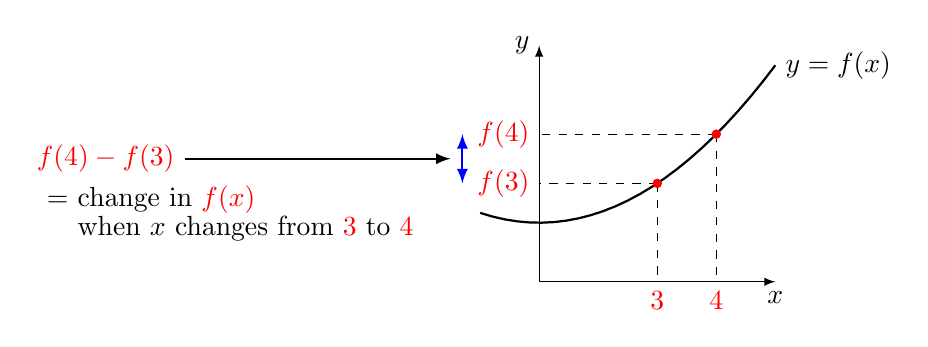
\begin{tikzpicture}[x=15mm,y=15mm,>=latex]
    \draw[thin,black,->] (0,0) -- (2,0) node[below] {$x$};
    \draw[thin,black,->] (0,0) -- (0,2) node[left] {$y$};
    \draw[thick,black] plot[domain=-0.5:2] (\x,{0.5+(\x)^2/3}) node[right] {$y=f(x)$};
    \draw[black,dashed] (1,{0.5+(1)^2/3}) -- (0,{0.5+(1)^2/3}) node[red,left] {$f(3)$};
    \draw[black,dashed] (1,{0.5+(1)^2/3}) -- (1,0) node[below,red] {$3$};
    \draw[black,dashed] (1.5,{0.5+(1.5)^2/3}) -- (0,{0.5+(1.5)^2/3}) node[red,left] {$f(4)$};
    \draw[black,dashed] (1.5,{0.5+(1.5)^2/3}) -- (1.5,0) node[below,red] {$4$};
    \filldraw[red] (1,{0.5+(1)^2/3}) circle (1.5pt);
    \filldraw[red] (1.5,{0.5+(1.5)^2/3}) circle (1.5pt);
    \draw[thick,blue,<->] (-0.65,{0.5+(1.5)^2/3}) -- (-0.65,{0.5+(1)^2/3});% node[midway,left,red] {$f(4)-f(3)$};
    \draw[thick,black,<-] (-0.75,{0.5+(1^2+(1.5)^2)/6}) -- (-3,{0.5+(1^2+(1.5)^2)/6}) node[left,red] {$f(4)-f(3)$};
    \node[right] at (-4.25,0.7) {$=$\ change in {\red$f(x)$}};
    \node[right] at (-4.25,0.45) {\phantom{$=$}\ when $x$ changes from
      {\red$3$}\ to {\red$4$}};
  \end{tikzpicture}
  \gap
  
  \uncover<2->{%
    \alert{Example:}\ 
    $f(x) = \text{stock value $x$ years after 2010}$ \\
    Ex: $f(3) = \text{stock value in 2013}$ 
    \bigskip

    $f(4)-f(3) = $\ \only<2>{?}\uncover<3->{change in stock value from
      2013 to 2014}
  }

}

\frame{
  \frametitle{Calculus is about change}

  The calculations involve limits.
  \halfgap

  \begin{enumerate}
    \setcounter{enumi}{9}
  \item What is the change in $f(x)=x^2$ between $2$ and $3$?
    \bigskip

    \begin{equation*}
      \text{A} = 1
      \qquad 
      \text{B} = 4 
      \qquad 
      \text{C} = 5 
      \qquad 
      \text{D} = 6
      \qquad 
      \text{E} = 9
      \qquad
      \pause
      \answer{C}
    \end{equation*}
    \gap

  \item What is the change in $f(x)=x^2$ between $2$ and $2+h$?
    \bigskip

    \begin{equation*}
      \text{A} = 2
      \qquad 
      \text{B} = h^2-2
      \qquad 
      \text{C} = 4h
      \qquad 
      \text{D} = h^2
      \qquad 
      \text{E} = 4h+h^2
      \qquad
      \pause
      \answer{E}      
    \end{equation*}
    \bigskip

    \alert{Note:}\ This \emph{exact}\ example comes up when we do calculus.

  \end{enumerate}


}

\section*{Summation}

\frame{
  \frametitle{\S5.3: Summation Notation}

  \begin{equation*}
    {\color{blue}\sum_{n={\red 1}}^{{\orange 7}}\ n}\  =\ {\red 1}+2+3+4+5+6+{\orange 7}
  \end{equation*}
  Read aloud: ``{\color {blue}The sum from n equals {\red 1} up to {\orange 7} of n}''\pause

  \begin{align*}
    \sum_{n={\red 1}}^{{\orange 4}}\ n^2
    & = {\red 1}^2+2^2+3^2+{\orange 4}^2 \\
    %
    \sum_{n={\red 1}}^{{\orange 5}}\ 2^n 
    & = 2^{\red 1}+2^2+2^3+2^4+2^{\orange 5}
  \end{align*}
  \pause

  {\color{blue} $\Sigma$} is  the Greek version of {\color{blue} S}\\
  \ \hspace*{0.5in}\ldots{}as in {\color{blue} S}ummation \\\pause
  \ \hspace*{0.5in}\ldots{}and the integral sign ${\color{blue}\int}$
  (Math 34B)


}

\frame{
  \frametitle{Examples:}

  \begin{enumerate}
    \setcounter{enumi}{7}
  \item $\displaystyle\sum^{{\orange 150}}_{k={\red 100}}\ (k^2+k)\  =\ ({\red 100}^2+{\red 100})+(101^2+101)\cdots+({\orange 150}^2+{\orange 150})$
    \gap
    \pause

  \item Summing entries in a table of data (or in a spreadsheet program)
    \begin{equation*}
      \sum_{p={\red 5}}^{{\orange 9}}\ x_p\ =\ x_{\red 5}+x_6+x_7+x_8+x_{\orange 9}
      \pause
    \end{equation*}
    \gap

  \item Summing values of a function
    \begin{equation*}
      \sum_{i={\red -2}}^{{\orange 1}}\ f(i)\ =\ f({\red -2})+f(-1)+f(0)+f({\orange 1})
    \end{equation*}

  \end{enumerate}


}


\frame{
  \frametitle{Examples 2: Averages}

  The {\color{blue}average} of $5,1,4,14$ is
  $$\frac{5+1+4+14}{4}$$\pause
  Add up the numbers you have then divide by how many numbers you had.
  \pause
  \gap

  Average of $x_1,x_2,\cdots,x_N$ is
  \begin{equation*}
    \frac{1}{N}\ \sum_{i=1}^N\ x_i\ =\ \frac{x_1+x_2+\cdots+x_N}{N}.
  \end{equation*}


}

\frame{
  \frametitle{Examples 3: Cool Sum Formulas}

  \begin{enumerate}
    \setcounter{enumi}{11}
  \item $\displaystyle{\color{blue}\left(\sum_{k=1}^{15}\ a_k\right)}
    +{\color{red}\left(\sum_{k=16}^{35}\ a_k\right)}\ =\ \sum_{k=1}^{35}\ a_k$
    \halfgap

    To see why this works, just write it out!\pause

    \begin{equation*}
      {\color{blue}(a_1+\cdots+a_{15})} + {\color{red}(a_{16}+\cdots+a_{35})}\ =\ (a_1+\cdots+ a_{35})
    \end{equation*}
    \pause
    \halfgap

  \item $\displaystyle{\color{blue}\left(\sum_{k=1}^{50}\ f(k)\right)}
    - {\color{red}\left(\sum_{k=20}^{50}\ f(k)\right)}\ =\ \sum_{k=1}^{19}\ f(k)$
    \pause
    \halfgap

    This just says
    \begin{equation*}
      {\color{blue}(f(1)+\cdots+f(50))} - {\color{red}(f(20)+\cdots+f(50))}\ =\ (f(1)+\cdots+ f(19))
    \end{equation*}

  \end{enumerate}


}


\frame{
  \frametitle{And More Cool Sum Formulas}

  \begin{enumerate}
    \setcounter{enumi}{13}
  \item $\displaystyle{\color{blue}\left(\sum_{i=1}^{7}\ a_i\right)}
    +{\color{red}\left(\sum_{i=1}^{7}\ b_i\right)}\ =\ \sum_{i=1}^{7}\ ({\blue a_i}+{\red b_i})$
    \pause
    \smallskip


    This just says that
    \begin{equation*}
      {\color{blue}(a_1+\cdots+a_7)}
      +{\color{red}(b_1+\cdots+b_7)}\ =\ ({\blue a_1}+{\red b_1})+\cdots+({\blue a_7}+{\red b_7})
    \end{equation*}
    \halfgap
    \pause

  \item $\displaystyle{\color{blue}\left(\sum_{i=1}^{100}\ p_i\right)}
    -{\color{red}\left(\sum_{i=1}^{50}\ p_i\right)}=$
    \bigskip

    \begin{equation*}
      \text{A} = \sum_{i=50}^{100}\ p_i
      \qquad
      \text{B} = \sum_{i=1}^{50}\ p_i
      \qquad
      \text{C} = \sum_{i=1}^{150}\ p_i
      \qquad
      \text{D} = \sum_{i=51}^{100}\ p_i
    \end{equation*}
    Hint: Just write it out!\pause\quad \answer{D}
    % \bigskip

    \begin{equation*}
      {\color{blue}(p_1+\cdots+p_{100})} -
      {\color{red}(p_1+\cdots+p_{50})}\ 
      =\ (p_{51}+\cdots+p_{100})
    \end{equation*}

  \end{enumerate}



}


% \frame{
%   \frametitle{One Last Question}

%   What is 
%   \begin{equation*}
%     \sum_{n=1}^3\ n+1\ =\ ?
%   \end{equation*}
%   \bigskip

%   \begin{equation*}
%     \text{A} = 6
%     \qquad 
%     \text{B} = 7
%     \qquad 
%     \text{C} = 8 
%     \qquad 
%     \text{D} = 9
%     \qquad 
%     \text{E} =10
%   \end{equation*}
%   \pause

%   {\color{red}\large{}WRONG!}
%   \smallskip\pause

%   It is {\red ambiguous} because it could mean two different things: 
%   \bigskip
%   \begin{equation*}
%     \left(\sum_{n=1}^3 n\right)+1 =7
%     \qquad\text{or}\qquad
%     \sum_{n=1}^3 (n+1) = 9.
%   \end{equation*}
%   \bigskip

%   Without parentheses, you get into trouble.
% }






\frame{
  \frametitle{That's it. Thanks for being here. }

  \begin{center}
    
\includegraphics[scale=.1]{Lecture 6 Picture.jpg}
  \end{center}
}










\end{document}


%%% Local Variables: 
%%% mode: latex
%%% TeX-master: t
%%% End: 
